% Faz com que o ínicio do capítulo sempre seja uma página ímpar
\cleardoublepage

% Inclui o cabeçalho definido no meta.tex
\pagestyle{fancy}

% Números das páginas em arábicos
\pagenumbering{arabic}

\chapter{Introdução}\label{intro}


\section{Motivação}\label{intro:historico}

\begin{refsection}

Esta tese surgiu da vontade de entender como os processos internos ao
organismo que produzem a variação em uma população interagem com os processos
evolutivos para dar origem à diversidade que observamos na natureza.
Resumidamente, nós procuramos estudar como a covariação genética se estabelece
e como ela evolui, e situamos essas questões dentro do contexto da
macroevolução de caracteres quantitativos. Para isso, nos valemos da teoria de
genética quantitativa na sua encarnação mais moderna, aliada a teoria de
evolução e das técnicas de mapeamento de loci de caracteres quantitativos.
Essa combinação permite estudar e prever as consequências das restrições
genéticas na evolução dos caracteres, e esmiuçar a arquitura genética por traz
dessas restrições. Nesta introdução, vamos revisar rapidamente a teoria de
genética quantitativa evolutiva e discutir a estrutura geral da tese. Neste
capítulo vamos utilizar as citações de forma esparsa, de forma a deixar o texto mais
fluido. A maior parte do contexto teórico pode ser encontrado em livros
básicos de evolução e genética, como~\textcite{Falconer1996-ot,
Lynch1998-ql, Barton2007-hq}. Alguns trechos mais avançados podem ser
encontrados em~\textcite{Rice2004-jf, Buerger2000-ez}. Argumentos que surgiram
em artigos específicos e são mais associados a essa referencia serão
apontados no texto.

\section{Variação genética e evolução} 

A variação fenotípica presente em uma população é fundamental para que a
evolução natural possa ocorrer. Em última instância, a variação fenotípica que
está disponível para que a evolução aconteça é consequência da variação
genética da população\footnote{A rigor variação genética não é estritamente
necessária, apenas variação \textit{herdável}. A herança cultural, por exemplo, pode
ser estudada com as ferramentas da evolução. Apesar disso, em populações
naturais, a maior parte da variação herdável é genética}. Essa variação
genética se dá no nível do DNA, com variantes discretas que segregam na
população. A informação genética contida nessas variantes é interpretada pelo
processo de desenvolvimento, e por meio de um sistema impossivelmente
complicado de interações, a cada geração um novo individuo é formado a partir
da informação no código genético. Mendel descreveu as leis que regem a herança
dessas variantes discretas estudando caracteres de herança discreta e simples,
ervilhas verdes ou amarelas, lisas ou rugosas. Mesmo esses caracteres simples,
cuja variação é determinada por um único locus do genoma, tem pro traz de si
um intrincado processo de desenvolvimento. Se para entender a evolução de
qualquer caráter, quanto mais caracteres complexos, fosse necessário um modelo
do processo que leva à sua formação, o estudo de evolução seria um iniciativa
que inviável. Felizmente, essa compreensão total do organismo não é
necessária. Para o estudo de evolução, basta um modelo de como os organismos
mudam. Somente a ligação entre variação genética e mudança fenotípica importa,
não o mecanismo por traz da formação do fenótipo. Se um gene está envolvido no
desenvolvimento de um caráter mas não apresenta variação genética, esse gene
não é importante para entender a evolução do caráter.

\subsection{Genética quantitativa} 

A grande maioria dos caracteres interessantes do ponto de vista evolutivo tem
uma base genética complexa. Tamanho corporal, sucesso reprodutivo, coloração,
forma, são todos caracteres cuja variação é determinada por muitos genes. Por
um lado, isso torna entender a arquitetura genética da variação desses
caracteres uma tarefa complicada, por outro lado, essa base complexa garante
que esses caracteres irão apresentar um padrão de variação contínuo, e
portanto pode ser estudados utilizando as ferramentas da genética
quantitativa. A variação continua que encontramos em caracteres complexos se
deve a dois fatores: a base poligênica e a variação ambiental a que os
fenótipos estão sujeitos. Quando vários genes estão envolvidos na determinação
de um caráter, a junção dos efeitos de herança particulada de cada umas das
variantes em cada um dos locus acaba por definir tantas classes de fenótipos
que a variação pode ser tratada como contínua. Além disso, se assumirmos que
cada gene contribui de forma aditiva ao fenótipo, o teorema do limite central
diz que a distribuição do caráter na população pode ser aproximado por uma
distribuição gaussiana. Na prática, a grande maioria dos caracteres de
interesse evolutivo podem ser aproximados por uma distribuição
normal\footnote{Interessantemente, a observação de que a distribuição
Gaussiana era tão ubíqua e útil na biologia evolutiva foi feita inicialmente
por um primo de Darwin, Francis Galton, em 1969}, ou transformados
trivialmente para uma distribuição normal\footnote{Caracteres contínuos que
são restritos a valores positivos, como distancias ou pesos, podem apresentar
uma distribuição log normal, em que o log das medidas tem distribuição normal.
Essa transformação implica que os genes tem efeitos multiplicativos no
fenótipo, e a transformação log transforma essas multiplicações em adições,
levando à distribuição normal após a transformação.}. Além disso, existe
diferenças ambientais no desenvolvimento de um caráter. Mesmo uma população de
indivíduos geneticamente idênticos irá apresentar alguma variação em seus
caracteres. Essa variação ambiental contribui para o aumento do número de
fenótipos possíveis e para a possibilidade de descrever a variação como
contínua (Fig.~\ref{discrete_aleles}).

\begin{figure}
    \centering
    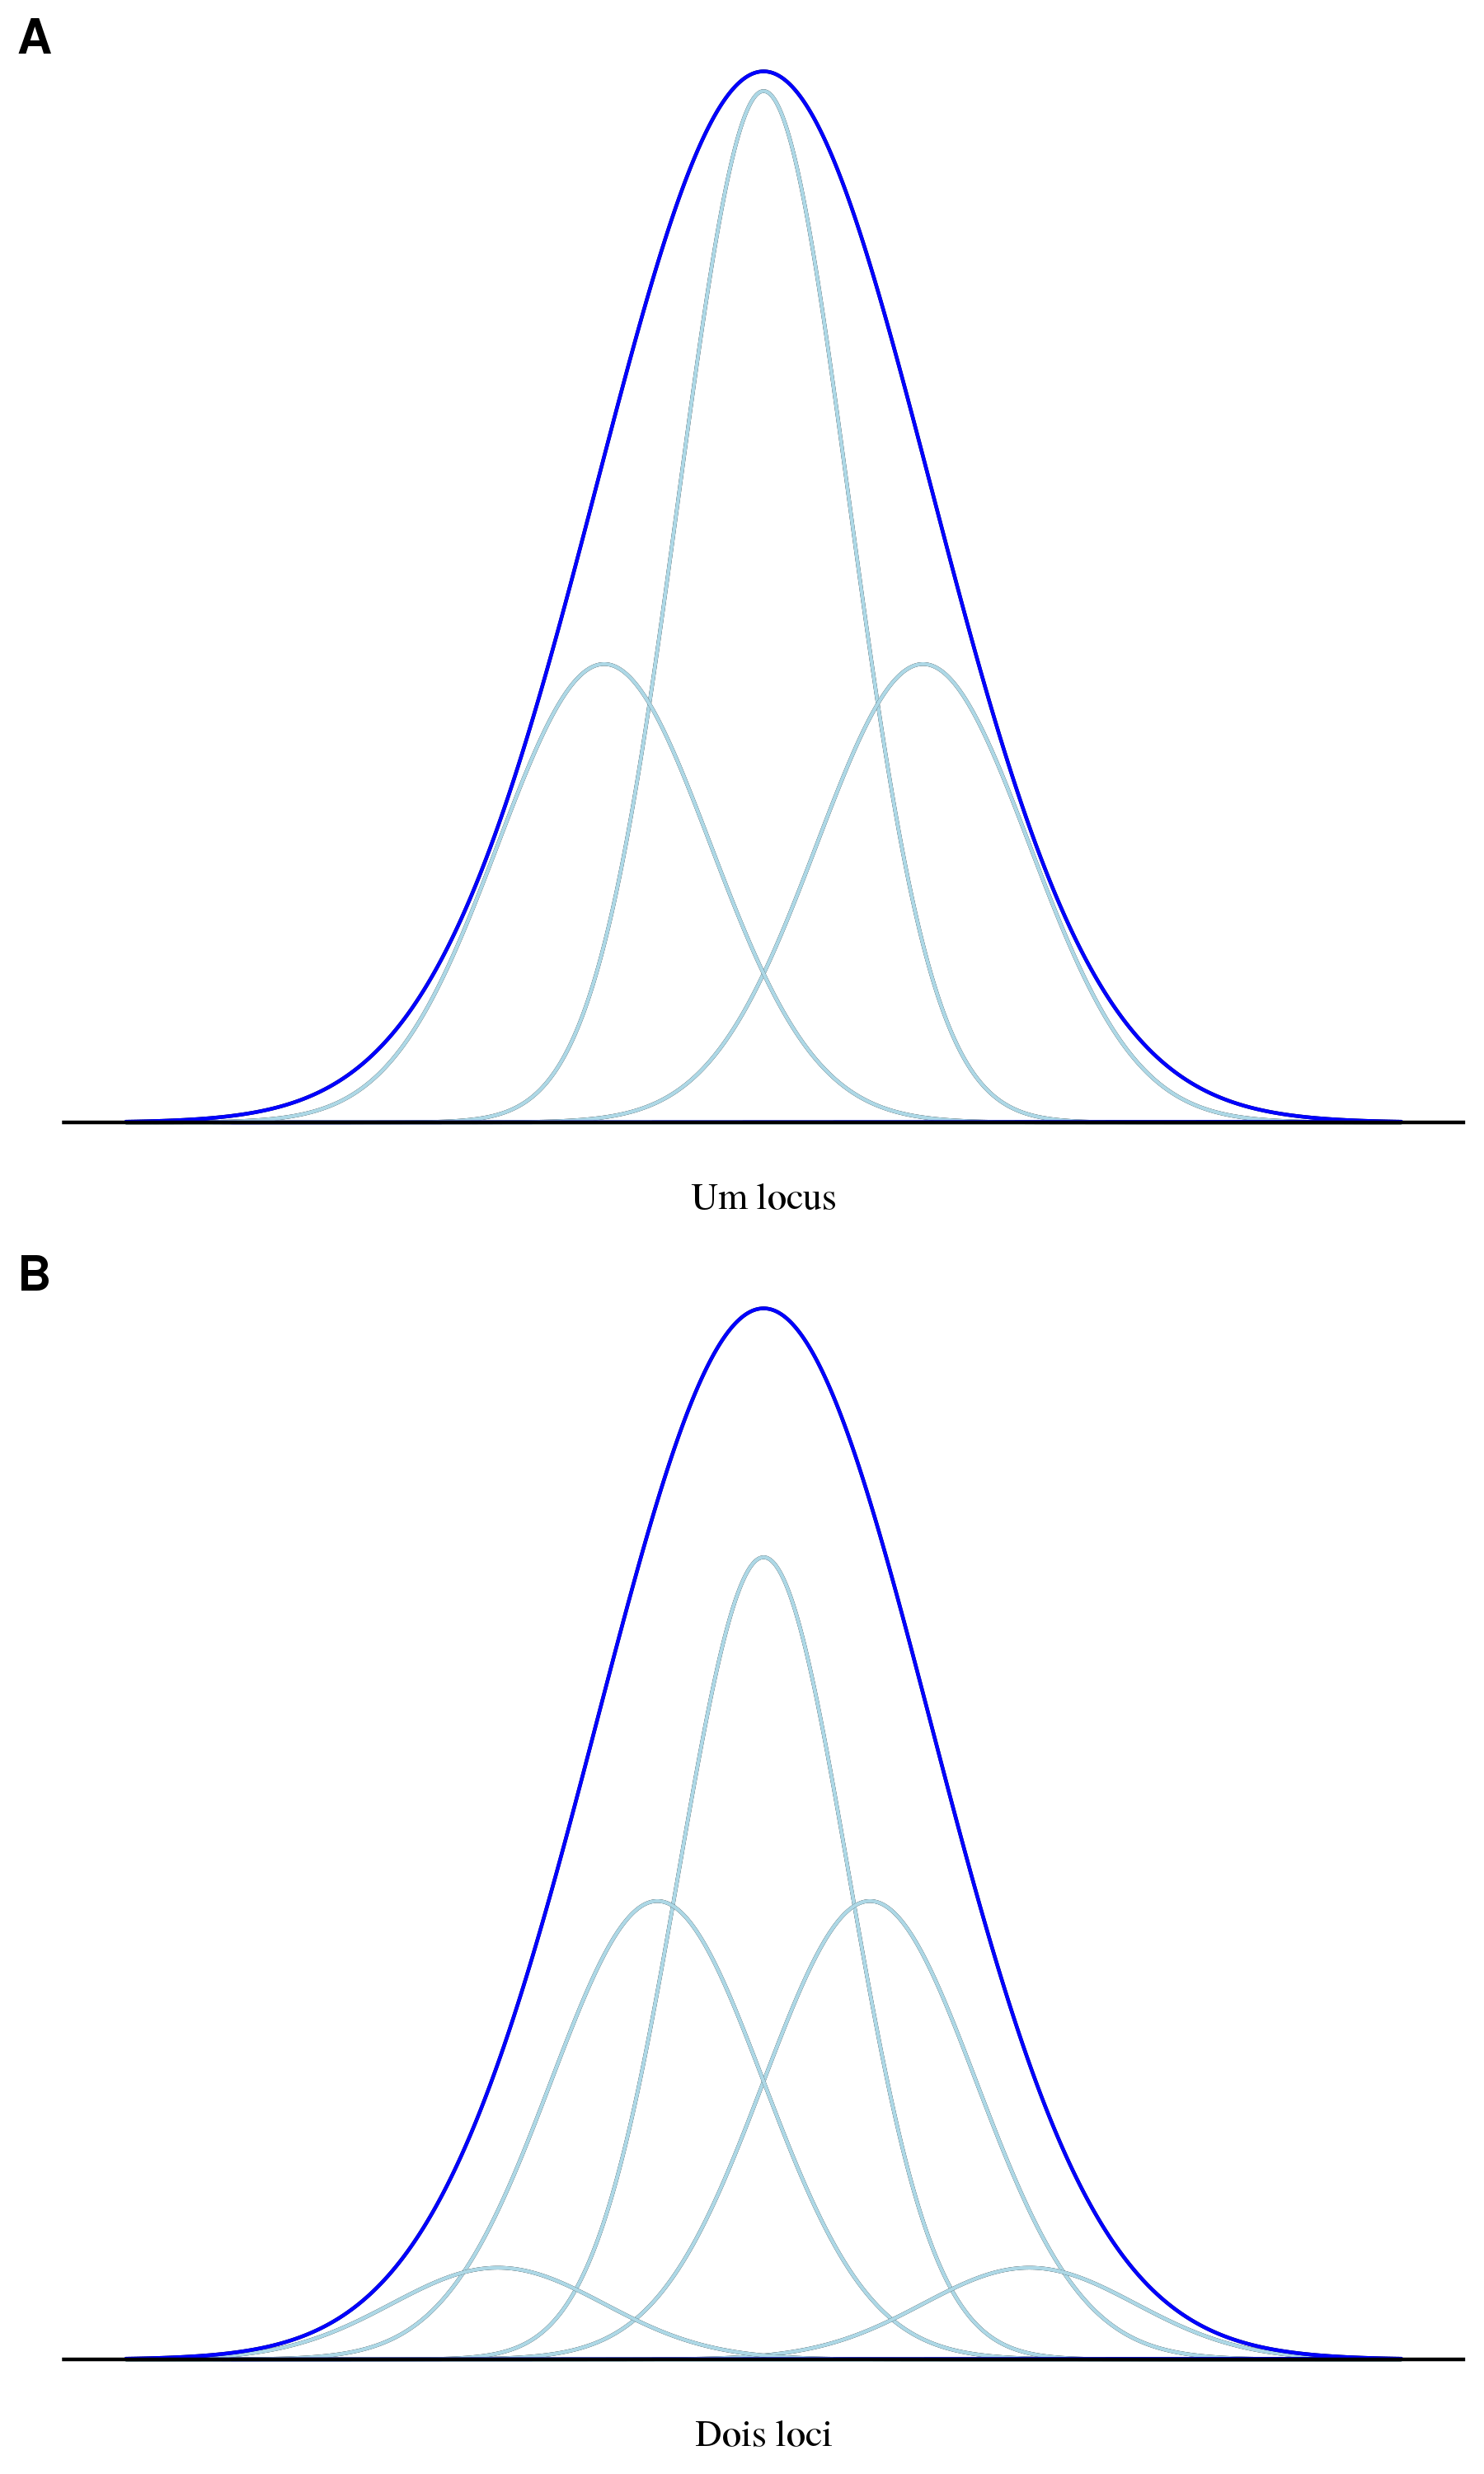
\includegraphics[width=300px]{discrete_gaussian.png}
    \caption[Variação contínua]{Mesmo com poucos loci, o modelo aditivo e variação ambiental são capazes de gerar distribuições fenotípicas muito próximas à gaussiana, dado que a diferença entre classes genotípicas seja da mesma escala da variação dentro de cada classe. A) Um loci aditivo com dois alelos de mesma frequência e a variação ambiental dentro de cada genótipo. As linhas finas mostram a variação dentro de cada classe, e a linha grossa a distribuição na população. B) Dois loci com dois alelos cada, com efeitos fenotípicos equivalentes. Adaptado de~\textcite{Barton2007-hq}.}
    \label{discrete_aleles}
\end{figure}

A ideia que a variação de um fenótipo pode ser expressa como a soma de vários
efeitos aditivos independentes, proposta por~\textcite{Fisher1930-bp}, é
central para a genética quantitativa. A primeira distinção é entre os
componentes devido a diferenças genéticas entre os indivíduos e o componente
devido a diferenças não genéticas (ambientais) da variação em uma população.
Para entender como o fenótipo é composto, podemos definir $G$ como a média do
fenótipo dos indivíduos que tem um determinado genótipo e $E$ como o desvio
devido ao ambiente. O fenótipo $P$ do indivíduo então é definido como:

\begin{equation}
P = G + E
\end{equation}

Como $G$ é definido como a média de $P$, a média de $E$ deve ser zero. Se a
distribuição de efeito ambientais for aproximadamente normal e se não existe
interação entre $E$ e $G$, ou seja, se a variação ambiental for a mesma para
todos os genótipos, um genótipo pode ser descrito apenas pelo seu valor
genotípico $G$ e pela sua variância ambiental $V_E$. Se a população em questão
é formada de indivíduos sexuados, o valor genotípico de um indivíduo será
composto pelas contribuições dos gametas parentais. Suponha que para os dois
locus que afetam um dado caráter o indivíduo tenha recebido um gameta $A_1B_1$
do pai e um gameta $A_2B_1$ da mãe. Então, o genótipo do indivíduo é
$A_1A_2B_1B_1$, heterozigoto no locus A e homozigoto no locus B. Dentro de um
modelo aditivo, no qual os efeitos de cada alelo são somados, o fenótipo do
indivíduo seria $P = \alpha_{A_1} + \alpha_{A_2} + 2\alpha_{B_1}$ + E, onde os
$\alpha$ representam as contribuições aditivas de cada alelo, que junto
compõem o valor genotípico do indivíduo. 

Naturalmente, o modelo puramente aditivo é uma simplificação enorme, e, na
prática, existem dois tipos de interações importantes entre alelos que podem
contribuir com o valor genotípico: interações de dominância, que acontecem
entre alelos do mesmo locus, e interações epistáticas, que acontecem entre
alelos em locus diferentes. Dominância acontece quando os efeitos dos alelos
em um locus não são simplesmente aditivos, ou, em outras palavras, quando o
heterozigoto não tem valor genotípico intermediário aos dois homozigotos
correspondentes. Já epistasia acontece quando o efeito de um alelo em um locus
depende do estado de outro locus. Ambas formas de interação são extremamente
comuns e contribuem de forma decisiva para mudança evolutiva, principalmente
epistasia, como veremos mais adiante.

Dentro do formalismo da genética quantitativa, as interações entre alelos e locus podem ser incluídas na formação do valor genotípico, também de forma aditiva. Então, a equação para o fenótipo de um indivíduo se torna:

\begin{equation}
P = G + E = A +D + I + E
\end{equation}

na qual nós decompomos o valor genotípico na sua porção devido aos efeitos
aditivos ($A$), de dominância ($D$) e epistáticos ($I$, interação). O termo
$A$ também é chamado de valor de acasalamento, e, além de ser a soma das
contribuições aditivas de cada alelo, este termo tem uma interpretação simples
que não faz referencia à base genética do fenótipo. O valor de acasalamento de
um indivíduo para um fenótipo pode ser definido como duas vezes a diferença
entre a média do fenótipo da sua prole com parceiros escolhidos ao acaso na
população e a média do fenótipo da população como um todo. A diferença é
dobrada pois o individuo contribui com metade do valor genotípico dos seus
filhos, a outra metade vindo ao acaso da população.

\subsection{Componentes da variação fenotípica}

Apesar de conceitualmente importantes, são raras as ocasiões em que temos
condição de medir valores dos componentes genotípicos de um indivíduo. Estimar
esse valores envolveria conhecer o genótipo de todos os indivíduos de uma
população em todos os locus que fossem de alguma forma envolvidos na formação
do fenótipo do indivíduo, uma tarefa praticamente impossível. A importância
prática desse esquema de decomposição fica mais clara quando consideramos a
variação população como um todo. A decomposição da variância da população nos
seus componentes devido a efeitos aditivos, de dominância e todos os outros
componentes do fenótipo pode ser feita sem nenhuma referencia à base genética
específica do fenótipo. Supondo que a variação genética e ambiental são
independentes, podemos expressar a variação fenotípica ($V_P$) como a soma das
variâncias genéticas e ambientais:

\begin{equation}
V_P = V_G + V_E
\end{equation}

Do mesmo modo, a variância dos valores genotípicos pode ser subdividida nos termos devido as diferentes tipos de efeitos genéticos:

\begin{equation}
V_G = V_A + V_D + V_I
\end{equation}

O componente da variância devido a diferenças nos valores de acasalamento
($V_A$) é chamado de variância genética aditiva, e tem um papel fundamental na
biologia evolutiva. O componente devido a interações epistáticas, $V_I$,
também pode ser subdivido em diferentes tipos de interação entre dois loci:
entre componentes aditivos ($V_{AA}$), entre componentes aditivos e de
dominância ($V_AD$), entre componentes de dominância ($V_DD$), e mesmo
componentes de grau mais alto, entre 3 ou mais loci. Essa subdivisão fornece
uma ferramenta poderosa para o estudo da variação e evolução em populações
naturais.

Cada um desses componentes pode ser estimado a partir da semelhança entre
indivíduos relacionado em uma população. Por exemplo, no caso da similaridade
entre pais e filhos, fundamental na herança de caracteres e para a evolução.
No caso mais simples, no modelo aditivo, o fenótipo de um indivíduo (filho) é dado por
$P_f = A + E_f$. O componente aditivo pode ser subdividido em duas partes, as
contribuições do pai e da mãe, então $P_f = A_1 + A_2 + E_f$. Já o fenótipo do pai
pode ser escrito como $P_p = A_1 + A_3 + E_p$, onde $A_1$ representa a porção
do valor de acasalamento compartilhada com o filho e $A_3$ a porção
independente do filho. A covariação entre pai e filho então é $cov(P_f, P_p) =
cov(A_1 + A_2 + E_f, A_1 + A_3 + E_p)$. A covariância da soma de fatores
independentes pode ser escrita como a soma das covariâncias par a par, então
$cov(P_f, P_p) = cov(A_1, A_1) + cov(A_1, A_3) + cov(A_2, A_1) + \cdots  +
cov(E_f, E_p)$. Como todos os componentes são independentes por construção, o
único termo que contribui para a covariância entre pais e filhos é $cov(A_1,
A_1) = var(A_1)$. Como a variância aditiva total é a soma das contribuições
paternas e maternas $V_A = var(A_1) + var(A_2)$, e como as contribuições
paternas e maternas são equivalentes, a covariância entre pais e filhos é a
metade da variância aditiva total ($cov(P_f, P_p) = var(A_1) = \frac{1}{2}V_A$).
A partir de deduções semelhantes, podemos estimar vários dos componentes da
variação genotípica a partir da covariância entre indivíduos relacionados. Por
exemplo, a variância de dominância pode ser estimada comparando a covariância
entre irmãos completos e pais e filhos, pois irmãos podem compartilhar
genótipos, enquanto pais não compartilham genótipos com os filhos. Então, na
presença de dominância, a covariância entre irmãos é maior que a covariância
entre pais e filhos.

\subsection{Herdabilidade e a resposta à seleção}

Para entender como se dá a resposta à seleção entre duas gerações, podemos
utilizar uma regressão linear entre a média dos pais e os filhos e imaginar
qual seria a resposta na geração dos filhos a um evento de seleção na geração
dos pais. No caso mais simples, de seleção por truncamento, podemos calcular a
nova média de pais e filhos após um evento de seleção no qual apenas casais
com média do fenótipo acima de um limiar de seleção deixam descendentes. Na
figura~\ref{PoR} podemos ver que a mudança na média na geração dos filhos será
dada pelo produto entre a inclinação da reta de regressão entre pais e filhos
e a mudança na média na geração dos pais. A solução de mínimos quadrados para
a inclinação da reta de regressão é dada pela covariância entre a variável
preditora e a resposta dividida pela variâncias da reposta. Já vimos que a
covariância entre pais e filhos é dada pela metade da variância aditiva, e a
covariância entre a média dos pais e filhos tem o mesmo valor, assumindo que a
covariância entre pais e filhos e mães e filhos é igual. Já o denominador, a
variância na média dos pais, pode ser calculada como:

\begin{equation}
var(\frac{P_{pais} + P_{\text{mães}}}{2}) = \frac{var(P_{pais}) + var(P_{\text{mães}})}{4} = \frac{V_P}{2}
\end{equation}

onde assumimos que a variância de pais e mães é igual. Então, a inclinação da
reta de regressão é igual à razão entre a variância aditiva e a variância
fenotípica total. Essa razão, a proporção da variação fenotípica que é devido
a variação aditiva, recebe um tratamento especial dentro da genética
quantitativa, recebendo o nome de herdabilidade ($h^2 =
\frac{V_A}{V_P}$).\footnote{O quadrado faz parte do simbolo, e se refere ao
fato da herdabilidade ser uma razão de variâncias, e portanto numa escala
quadrática.}

\begin{figure}
    \centering
    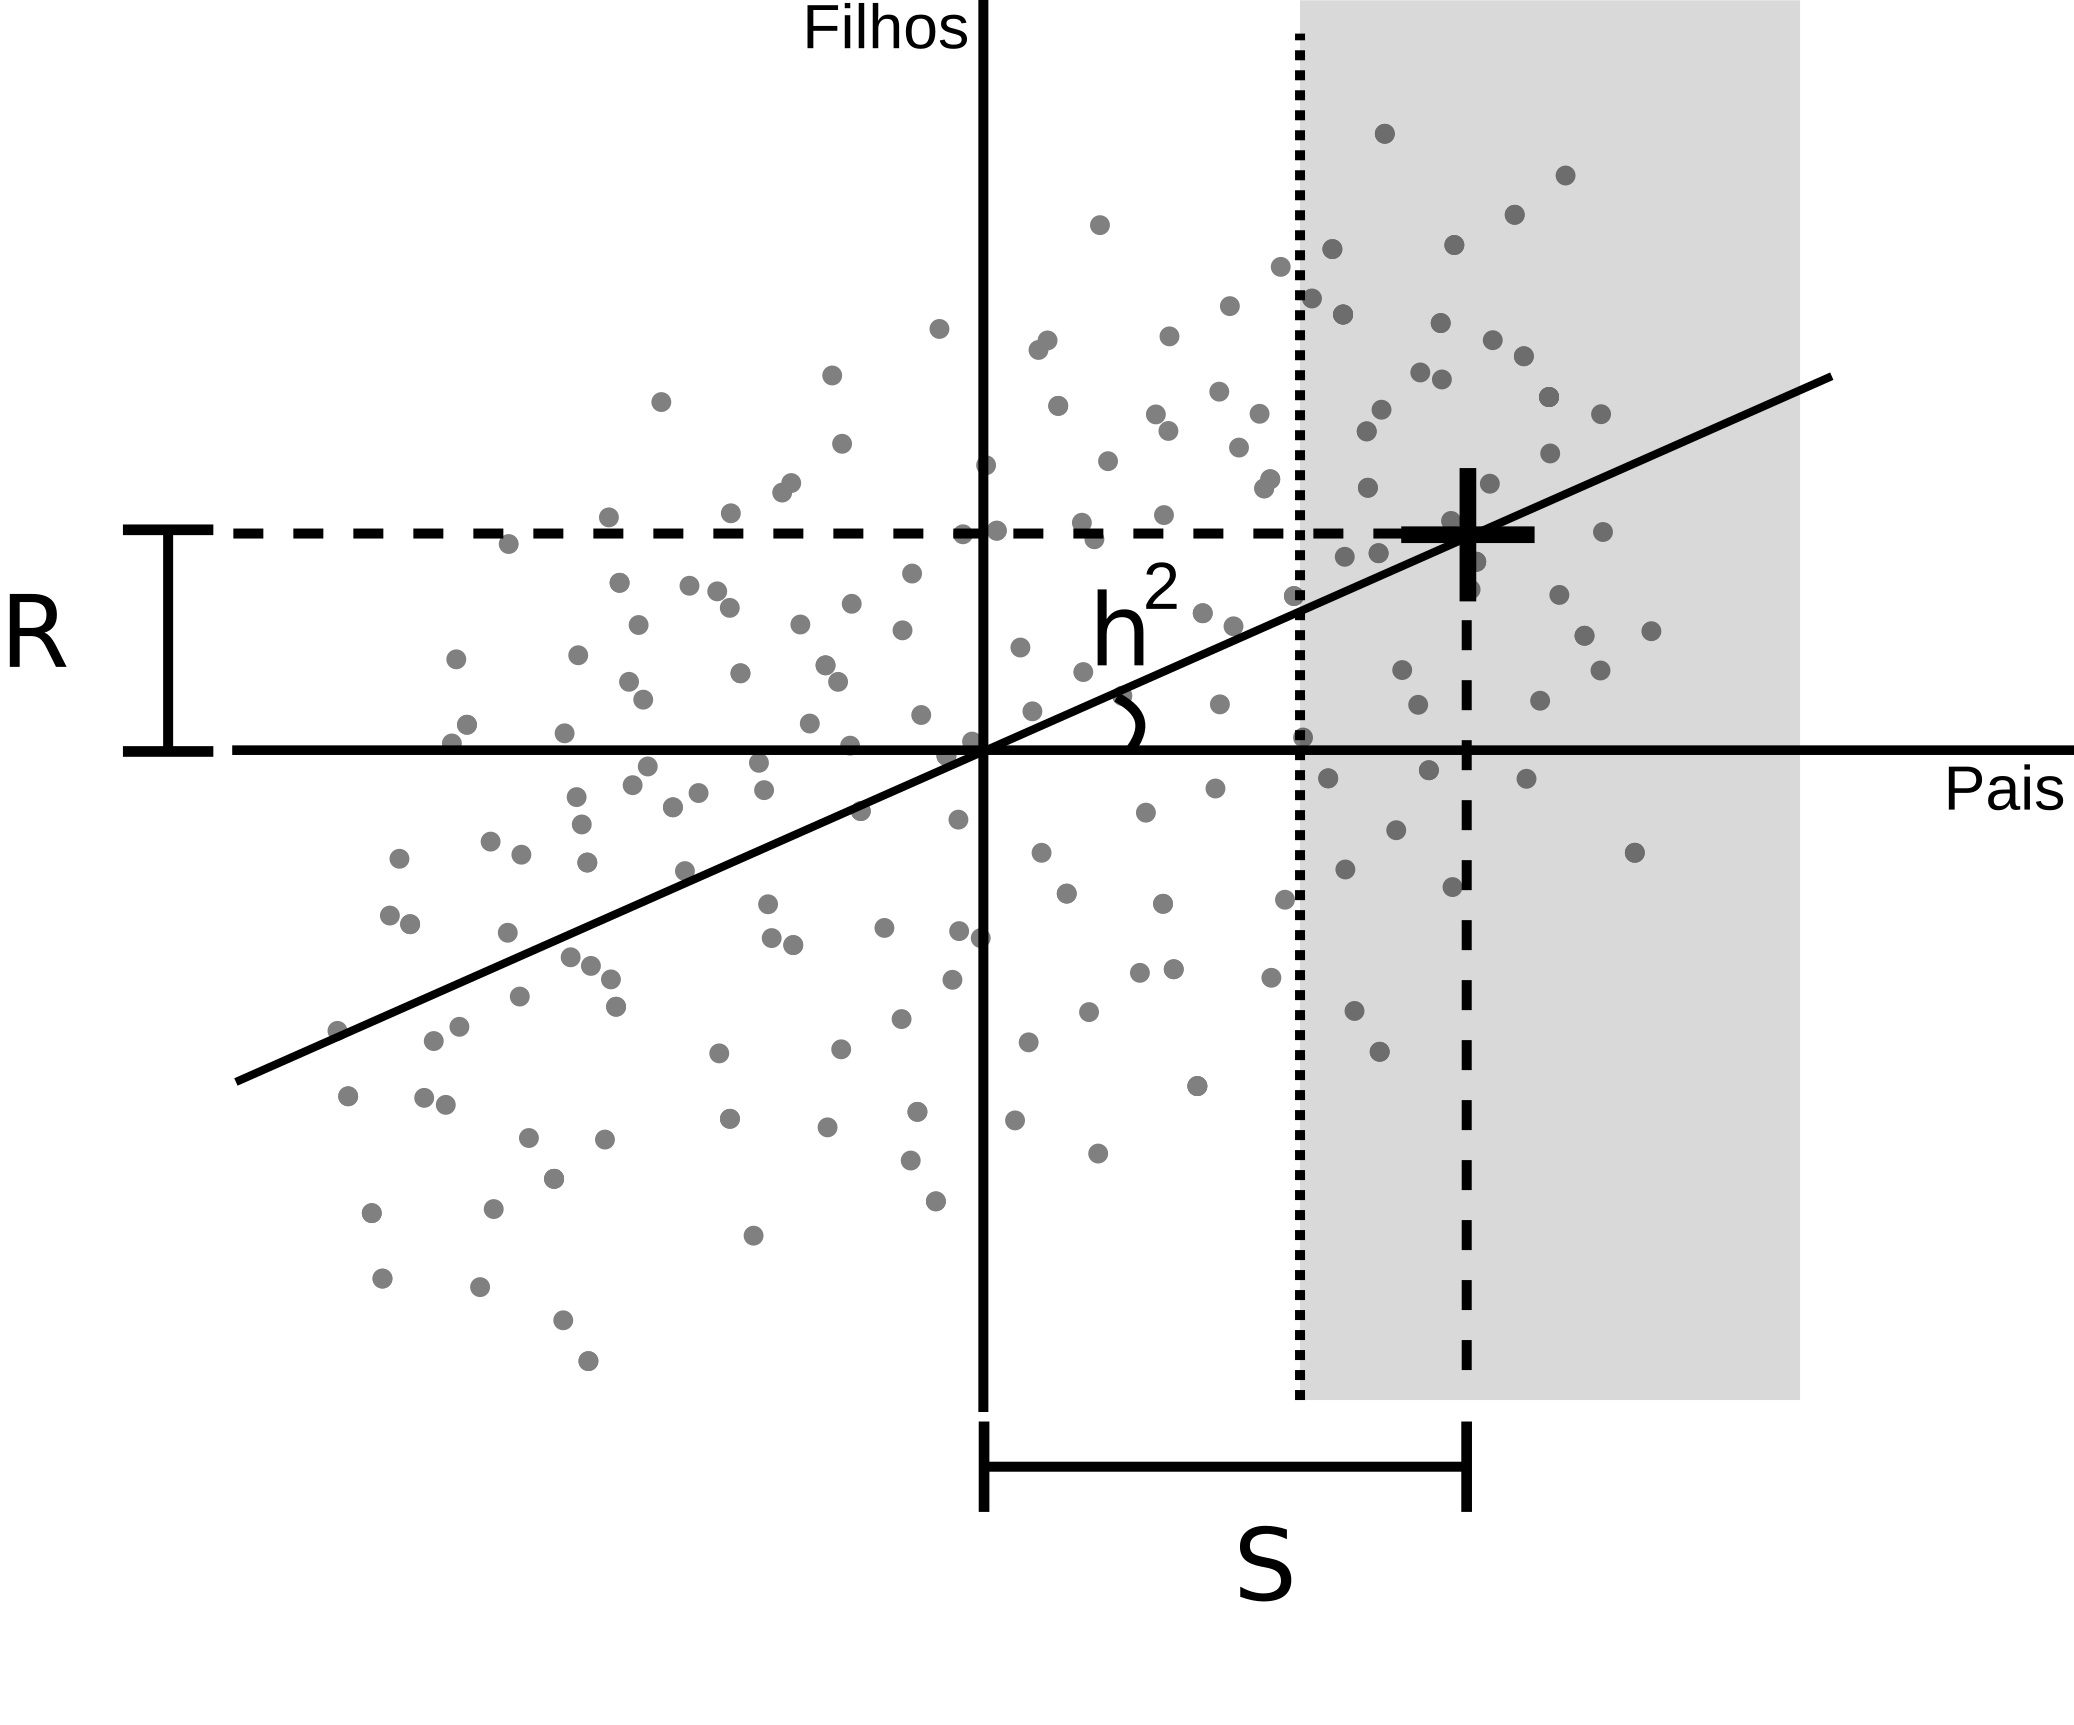
\includegraphics[width=350px]{parent-offspring.png}
    \caption[Regressão pais e filhos]{Regressão do fenótipo dos filhos na média 
    do fenótipo dos pais permite prever a resposta à seleção direcional, em
    que a média da população em uma geração é alterada por um evento de
    seleção. Neste caso, aplicamos um limiar de seleção na geração parental, e
    apenas casais com média do fenótipo maior que o limiar (na região
    sombreada) deixam descendentes, a cruz escura marca a nova média após a
    seleção. A mudança na média da geração dos pais após o evento de seleção é
    medida pelo diferencial de seleção $S$. Essa mudança na média causa uma
    resposta evolutiva ($R$) na média da geração dos filhos que pode ser
    predita utilizando uma regressão linear. A inclinação da regressão é dada
    pela covariância entre pais e filhos e a variância fenotípica na geração
    parental. Em condições bastante gerais, a inclinação da reta de regressão pode ser 
    estimada como a razão entre a variância aditiva e a variância fenotípica, a
    herdabilidade ($h^2$).}
    \label{PoR}
\end{figure}

Esse tratamento de regressão nos mostra como a herdabilidade é especialmente
importante para entender a resposta evolutiva, pois é a ela que determina como
uma mudança na média dos pais se traduz numa mudança evolutiva na média dos
filhos. Essa relação é dada pela equação do criador, que relaciona a mudança
em um fenótipo de uma geração para outra ($R$) com a mudança dentro de uma
geração devido a um episódio de seleção (o diferencial de seleção, $S$):

\begin{equation}
R = h^2S = \frac{V_A}{V_P}S	
\end{equation}

A intensidade de seleção é medida pelo diferencial de seleção, e quanto maior
a mudança na média dentro de geração maior será a mudança entre gerações. Além
disso, a equação do criador nos mostra que a resposta à seleção depende não só
da intensidade de seleção, mas também depende fundamentalmente da presença de
variação aditiva. Sem variação aditiva, sem herdabilidade, não há como haver
resposta na próxima geração, e quanto maior a herdabilidade maior será a
resposta a seleção.

\subsection{Resposta à seleção multivariada}

Se estamos interessados em fenótipos complexos, compostos de muitos
caracteres, além de quantificar a variância individual de cada um, podemos
também levar em conta a interação entre eles. De forma análoga à variância, a
covariância mede a variação conjunta de dois caracteres. A matriz de
covariância genética aditiva (matriz G) representa na diagonal as variâncias
genéticas aditivas dos caracteres, e fora da diagonal a covariância entre os
valores de acasalamento de caracteres diferentes. Já a matriz de covariância
fenotípica (matriz P) reune as variância e covariâncias entre os fenótipos da
população.

Usando essas matrizes é possível escrever o análogo multivariado da equação do
criador, a equação de resposta multivariada de~\textcite{Lande1979-by}, que
tem essencialmente a mesma forma:

\begin{equation}
\Delta \mathbf{\overline z} = GP^{-1}\mathbf{S} = G\beta
\end{equation}

Nesse caso, tanto a resposta à seleção ($\Delta \mathbf{\overline z}$) quanto
o diferencial de seleção ($\mathbf{S}$) são representados por vetores, sendo
que cada componente representa um caráter analisado. Frequentemente, o termo
$P^{-1}S$ é representado por $\beta$, o gradiente de seleção. O uso do
gradiente de seleção é conveniente por algumas razões. Primeiro, o vetor
$\beta$ possui uma interpretação geométrica simples, representando a direção
fenotípica de maior aumento da aptidão\footnote{Dai o nome \textbf{gradiente},
que no cálculo diferencial é definido como o vetor de derivadas que aponta a
direção de maior mudança em uma superfície multivariada.}; segundo, o
gradiente de seleção já desconta as covariâncias fenotípicas e permite inferir
quais caracteres estão efetivamente sob seleção.\footnote{Isso só vale caso
todos os caracteres relevantes para a aptidão estejam inclusos na análise.}

Se as matrizes P e G forem diagonais, ou seja, se todas as covariâncias entre
valores de acasalamento e entre fenótipos forem nulas, a equação de Lande se
resume a várias instâncias da equação do criador. Porém, caso as covariâncias
não sejam nulas, a equação de Lande prevê uma resposta indireta à seleção
mesmo em caracteres que não estão sobre seleção, caso eles sejam
correlacionados com caracteres que estão sobre seleção. Para entender esse
efeito indireto, podemos considerar o caso com dois caracteres, em que a
equação de Lande é:

\begin{equation}
G\beta  =
\left (
\begin{matrix}
G_{11} & G_{12} \\
G_{21} & G_{22} \\
\end{matrix}
\right )
\left (
\begin{matrix}
\beta_{1}  \\
\beta_{2}   \\
\end{matrix}
\right )
=
\left (
\begin{matrix}
G_{11}\beta_{1} +  G_{12}\beta_{2} \\
G_{21}\beta_{1} +  G_{22}\beta_{2} \\
\end{matrix}
\right )
=
\left (
\begin{matrix}
\Delta z_{1}  \\
\Delta z_{2}   \\
\end{matrix}
\right )
=
\Delta z
\end{equation}

Os termos $G_{11}\beta_{1}$ e $G_{22}\beta_{2}$ representam a resposta à
seleção direta em cada caráter. Mas além dos termos diretos, temos também  os
termos indiretos $G_{12}\beta_{2}$ na resposta do caráter $z_1$ e
$G_{21}\beta_{1}$ na resposta do carácter $z_2$, que dependem da seleção no
outro caráter e na covariância genética entre caracteres. A presença de
respostas indiretas a um gradiente de seleção faz com a resposta observada
($\Delta z$) não seja na mesma direção do gradiente de seleção. Esse desvio da
resposta evolutiva em relação à seleção direcional é considerado um tipo de
restrição genética, e pode ter consequências importantes na diversificação.

\section{Estrutura da variação genética}

A influência da covariação genética na resposta à seleção implica que conhecer
o padrão e intensidade da covariância genética é fundamental para o estudo de
evolução. O padrão de covariância genética se refere à organização da
covariação, quais caracteres são mais relacionados, quais grupos tem
covariâncias positivas ou negativas, quais caracteres compõem um grupo de
covariâncias altas, etc. Já a intensidade se refere à magnitude total das
covariâncias. Como as covariâncias são medidas na escala dos caracteres, é
comum utilizar uma medida de associação padronizada, que permita a comparação
da intensidade de associação entre caracteres de tamanhos e escalas de
variação diferentes. A medida usual é a correlação entre caracteres, definida
como a covariância dividida pelo produto dos desvios padrões dos caracteres em
questão. Tanto o padrão quanto a intensidade das correlações genéticas são temas
centrais desta tese.

O padrão de correlação genético é principalmente definido pela arquitetura
genética dos caracteres. Genes pleiotrópicos, que afetam mais de um caráter, e
desiquilíbrio de ligação, a herança conjunta de alelos específicos, contribuem
para a covariância genética e provocam respostas correlacionadas. Em uma
parcela significativa dos sistemas biológicos, da expressão gênica à
morfologia, a organização da covariação genética se dá de forma modular. Em
uma organização modular podemos perceber conjuntos de caracteres mais
correlacionados entre si do que com o restante do
organismo.~\textcite{Olson1958-qk} notaram como esses grupos de caracteres
frequentemente estão envolvidos no desempenho de uma função especifica e estão
também associados pelo desenvolvimento, compartilhando uma origem embriológica
ou sendo formados pelas mesmas vias de desenvolvimento.

A organização modular é essencial para que a evolução possa acontecer, por
criar uma certa independência entre os caracteres. Em última instância, a
própria existência de caracteres identificáveis é uma evidencia para a
importância da organização do organismo em módulos relativamente
independentes.~\textcite{Wagner1996-ui} foram pioneiros no entendimento da
modularidade como uma adaptação para permitir que os organismos tivessem a
capacidade de responder a seleção de forma eficiente, e nesse contexto apresentam
modularidade como uma solução a uma série de problema que os organismos estão
sujeitos ao interagir com os processos evolutivos, como a necessidade de
evolução coordenada de caracteres funcionalmente ligados e a robustez a
mudanças em outras partes do organismo.

\subsection{Evolução da covariação genética}

A evolução da covariação genética é o tema central desta tese, e pensar no
padrão de covariação como uma adaptação exige entender como a variação
genética entre indivíduos contribui para variação do próprio padrão de
covariação, para que o padrão de variação possa evoluir. Por um lado, é claro
que a variância aditiva pode mudar ao longo do tempo pela simples mudança na
frequência de alelos aditivos. Por exemplo, uma população que perde variação
genética por endocruzamento pode  perder toda a variação genética se novos
alelos não forem introduzidos por mutação, e isso obviamente mudaria o padrão
de covariação genética, pois não haveria variação. Na pratica isso é
extremamente raro na natureza, e a grande maioria dos caracteres apresentam
variação genética suficiente para responder à seleção. Além disso,
empiricamente podemos observar uma certa constância nos padrões de covariação
genética em uma escala de tempo evolutivo, mesmo que existam flutuações de
curto prazo. De alguma forma, não só a variação genética é mantida em níveis
consideráveis, mas a estrutura dessa variação parece ser adaptativa e
relativamente estável, com padrões modulares associados ao desempenho de
funções. Como essa variação é mantida e como os padrões são estabelecidos e
mantidos é um problema fundamental em biologia evolutiva.

A manutenção da variação genética aditiva foi durante os últimos 30 anos e
continua sendo um tema absolutamente central em biologia evolutiva. Não vamos
abordar este tema diretamente, mas cabe fazer um breve comentário sobre os
processos que mantém a variação genética. A genética quantitativa assume que
exista variação aditiva suficiente para responder à seleção, e no geral essa
hipótese é bastante razoável. A imensa maioria dos caracteres e combinações de
caracteres apresentam variação genética apreciável, mesmo em sistemas
multivariados e sujeitos a seleção natural. Um exemplo interessante de um
teste empírico da capacidade de um sistema multivariado de responder à seleção
em qualquer direção foi feito por~\textcite{Hine2014-ps}, e os resultados
foram típicos: todas as direções do espaço fenotípico tem variação suficiente
para responder à seleção. Vários processos contribuem para essa manutenção de
variação, como migração, sobre dominância na aptidão, efeitos antagonistas de
alelos na aptidão ao longo da vida, variação espacial na superfície de
seleção. Todos esses processos são importantes, mas, o processo mais
importante para a manutenção da variação e, em última instância, de onde vem
toda variação é a mutação. De alguma forma, o influxo de novas variantes por
mutação equilibra a remoção de variação por mutação e seleção. A forma exata
desse equilíbrio não é bem entendida, e diferentes aproximações levam a
expectativas diferentes para a taxa de mutação necessária para a manutenção da
variação em níveis razoáveis e para o número de loci envolvidos na produção da
variação de caracteres fenotípicos, mesmo para modelos aditivos simples. A
inclusão de complicações como epistasia e pleiotropia também não fornece um
quadro claro do equilíbrio entre mutação e seleção, apesar de que interações
epistáticas parecem ser uma fonte importante e ainda mau documentada de
variação aditiva. Em resumo, a maioria dos modelos prevê menos variação
aditiva do que nós observamos dadas as taxas mutacionais, e é interessante
como o problema da teoria evolutiva é justamente que a seleção pode ser mais
efetiva que o previsto pelos modelos.

A segunda questão, referente a origem e manutenção padrão da variação
genética, é mais recente, e estamos agora entendendo como os efeitos genéticos
e o processo de desenvolvimento permitem evolução nos padrões de covariação.
Em particular, interações epistáticas tem se mostrado fundamentais para a
geração de variação nos padrões de covariação, fornecendo um mecanismo para a
alterações de padrões pleiotrópicos (para uma revisão recente
veja~\textcite{Pavlicev2015-up}). A abundância dessa variação epistática
garante que os padrões podem efetivamente evoluir em populações naturais. Além
disso, variação epistática pode também afetar o padrão mutacional de um gene,
e  novas mutações que afetem mais de um caractere tem o potencial de criar ou
remover correlações entre caracteres. Na presença de seleção estabilizadora,
existe uma expectativa teórica de que os padrões de correlação mutacional,
genético e seletivo se alinhem, mantendo o padrão de covariação
estável~\parencite{Cheverud1984-mi}. Em populações naturais, foi documentada
tanto a manutenção de padrões de covariação em escala macro
evolutiva~\parencite{Marroig2001-ne}, quanto a mudanças adaptativas nos
padrões de covariação~\parencite{Young2005-nk}. Quais os mecanismos seletivos,
genéticos, mutacionais e de desenvolvimento envolvidos na alteração ou
manutenção dos padrões de covariação ainda é uma questão em aberto em biologia
evolutiva.

Nesta tese, abordamos a questão da evolução e manutenção dos padrões de
covariação utilizando diversas populações experimentais submetidas a regimes
de seleção diferentes, simulações computacionais e técnicas estatísticas
modernas para ligar os efeitos genéticos à covariação e entender o efeito da
seleção na covariação genética e nos padrões pleiotrópicos.

\section{Esquema da Tese} 

Esta tese é apresentada em cinco capítulos relativamente independentes mas
ligados pelo tema da evolução da covariação genética. Com exceção do Capitulo
5, que depende do Capítulo 4 em alguns passos técnicos, todos podem ser lidos
independentemente. 

O Capitulo 2 (\textit{How does modularity in the genotype-phenotype map shape
development and evolution?}) apresenta uma revisão básica do conceito de
modularidade e discute as causas e consequências da organização modular da
arquitetura genética. Este capitulo pode ser visto como uma segunda
introdução, mais técnica e motivadora dos capítulos experimentais que o seguem.

O Capítulo 3 (\textit{The Evolution of Phenotypic Integration: How directional
selection reshapes covariation in mice}) aborda o problema da evolução da
intensidade da correlação fenotípica e genética após um episódio de seleção
direcional. Utilizando camundongos provenientes de um experimento de seleção
artificial para alteração do peso corporal, nós medimos o padrão e a
intensidade de correlação em caracteres cranianos em duas linhagens
selecionados para aumento de tamanho, duas linhagens selecionadas para
diminuição de tamanho, e uma linhagem controle. Nossos resultados mostram que
o padrão de covariação muda com a seleção direcional, aumentando a proporção
de variação alinhada com a seleção direcional, e portando aumentando a
evolvabilidade relativa na direção de seleção. Este capítulo foi escrito em
colaboração e tem Anna Penna como co-primeira autora. Os dados foram derivados
de um projeto de iniciação científica realizado no laboratório de evolução de
mamíferos, e os animais utilizados no projeto foram cedidos pela professora
Maria Inés Oyarzabal da Universidade de Nacional de Rosário, Argentina. O
capítulo foi publicado na revista \textit{Evolution} (doi:10.1111/evo.13304).

O Capítulo 4 (\textit{Genomic Perspective On Multivariate Variation,
Pleiotropy, And Evolution}) utiliza uma população intercruzada de camundongos
provenientes de duas linhagens puras para estudar como o padrão de efeitos
genéticos se relaciona com o padrão de covariação de um conjunto de caracteres
da curva de crescimento. As linhagens puras são derivadas de dois experimentos
independentes de seleção no peso corporal, um para aumento de peso e um para
diminuição de peso. Utilizando técnicas de mapeamento genético e a teoria de
genética quantitativa, nós fomos capazes de particionar o efeito dos
componentes aditivos e de dominância na covariação genética, e mostramos que o
padrão de covariação genética é o resultado da combinação da influência da
seleção e de restrições internas que moldam os efeitos pleiotrópicos. Além
disso, nós também comparamos duas técnicas de mapeamento genético na sua
capacidade de inferir o fenótipo das linhagens puras utilizando somente os
efeitos genéticos na população intercruzada. 

O Capítulo 5 (\textit{Genetic Architecture and the Evolution of Variational
Modularity}) aplica os mesmos métodos desenvolvidos no capítulo anterior para
relacionar efeitos genéticos com a covariação em uma linhagem intercruzada de
camundongos formada por seis linhagens puras advindas de um experimento de
seleção direcional para a alteração da curva de crescimento. Nesse experimento
de seleção artificial, foi observado uma mudança marcante no padrão de
covariação genéticas após a seleção, com a eliminação de uma correlação
positiva entre as fases iniciais e finais do crescimento. Utilizando a
população intercruzada, nós exploramos a base genética do novo padrão de
covariação e relacionamos esse padrão e os feitos genéticos com a história
evolutiva das linhagens selecionadas. Além disso, utilizamos simulações baseadas
em indivíduos para estabelecer expectativas sobre a distribuição de efeitos

O Capitulo 6 (\textit{Modularity: Genes, Development, and Evolution}) é uma
revisão abordando tanto as bases genéticas do padrão de covariação quanto sua
evolução e as consequências macro evolutivas da covariação genética. Sendo uma
revisão bastante geral, o capítulo funciona como uma introdução relativamente
completa e como uma discussão das consequências dos temas abordados nos
capítulos experimentais anteriores, mais específicos. Este capítulo foi escrito em
colaboração e tem Arthur Porto como co-primeiro autor. O capítulo foi
publicado na revista \textit{Annual Review of Ecology, Evolution, and
Systematics} (doi:10.1146/annurev-ecolsys-121415-032409).


\printbibliography


\end{refsection}